\usetikzlibrary{angles, quotes}



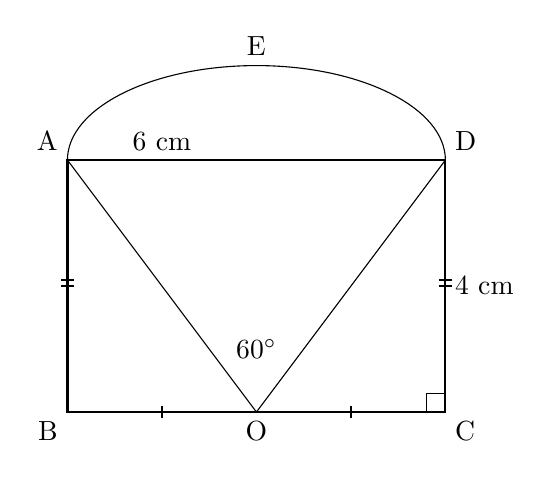
\begin{tikzpicture}[scale=0.8]
    % Rectangle ABCD
    \draw[thick] (0,0) coordinate (B) -- (6,0) coordinate (C) -- (6,4) coordinate (D) -- (0,4) coordinate (A) -- cycle;
    
    % Midpoint O on BC
    \coordinate (O) at (3,0);
    
    % Sector/Triangle lines
    \draw (A) -- (O) -- (D);
    
    % Arc AED (centered at O)
    \draw (6,4) arc (0:180:3 and 1.5); % Approximate curve for AED
    
    % Labels
    \node[below left] at (B) {B};
    \node[below right] at (C) {C};
    \node[above right] at (D) {D};
    \node[above left] at (A) {A};
    \node[below] at (O) {O};
    \node[above] at (3,5.5) {E};
    
    % Measurements
    \node[above] at (1.5,4) {6 cm};
    \node[right] at (6,2) {4 cm};
    \draw (3,1) node {$60^\circ$};
    
    % Markings (midpoint and equality)
    \draw[thick] (1.5,-0.1) -- (1.5,0.1); % tick on BO
    \draw[thick] (4.5,-0.1) -- (4.5,0.1); % tick on OC
    \draw[thick] (-0.1,2) -- (0.1,2); \draw[thick] (-0.1,2.1) -- (0.1,2.1); % ticks on AB
    \draw[thick] (5.9,2) -- (6.1,2); \draw[thick] (5.9,2.1) -- (6.1,2.1); % ticks on CD
    
    % Right angle at C
    \draw (5.7,0) -- (5.7,0.3) -- (6,0.3);
\end{tikzpicture}